\chapter{Analysis}

Now that we have described the game's design, in this chapter, we will explain the approach we took to implement it from a high-level perspective.
We will provide concrete details only for what will be implemented in the playable demo version, but as always, we will make many decisions based on the original vision of our game.

\section{Game Engine}

Game engines provide many important and useful systems for us, so we can focus on implementing the game logic.
For our game, we chose Unity because it offers all the features we need, and the author is already familiar with it.
There are many game engines we could have used, and the high-level decisions presented in this chapter would be still applicable.
However, in some sections we will use nomenclature that is specific to Unity, so we assume the reader is at least familiar with it.
More information is available in the official documentation~\cite{UnityDocs}.

\section{Procedural Generation}

As explained in the previous chapter, a lot of the game will be procedurally generated including the map of a run and each battle along the way.
From the player's perspective, all this and the rewards they receive will be randomized and unpredictable.
However, each run will have a single seed that deterministically decides all the \enquote{random decisions} the game makes.
Two runs with the same seed should look identical and if the player makes the same decisions and choices, the outcomes should be the same.
This allows the players to share seeds of the runs they found interesting and compare their skill in the same situations.
Furthermore, this is helpful for debugging, because it lets us easily reproduce any issue with the generation just by running it with the same seed.

We want to allow the player to save the game between battles.
Here, determinism is also useful, because it allows us to save just the seed of something that was generated, instead of saving it whole, which leads to simpler and smaller save files.

\subsection{Random Number Generators}

Randomized algorithms, like the ones we will use for procedural generation, depend on a \emph{random number generator} as their source of randomness.
A \textbf{random number generator} (or \emph{RNG}) produces a sequence of numbers that looks random and is unpredictable.
They are well explained in \citetitle{johnston2018random}~\cite{johnston2018random} by David Johnston.
Some RNGs use specialized hardware to generate truly random data using an external source of entropy, these are called \emph{true random number generators}.
However, we want a \emph{deterministic RNG}, also known as a \emph{pseudorandom number generator} (\emph{PRNG}).
These produce the random data using a completely deterministic algorithm, but unless we know the current internal state of the generator, the outputs still can't be predicted.
The initial state of a PRNG is called the \emph{seed}, and a generator will always generate the same sequence of outputs when \emph{seeded} with the same value.

Each query advances the generator's state, so the value a deterministic random number generator returns depends on the number of previous requests.
If we used one generator for generating everything, the outcomes of different systems would depend on the order they were generated in.
For example, when a player triggers some effect that uses randomness \emph{before} generating a level, the level would be different than if the player triggered the randomized effect \emph{after} the level was generated.
To remedy this, we will utilize a simple trick we call \emph{seed branching} all throughout the procedural generation.
Whenever we want more systems to be independent of each other, we create a new RNG instance for each system, and we seed them with each with a seed generated from the old RNG in advance.
For example, we will have a master RNG seeded with the seed of the run, from which we will generate the seeds for the map generator, reward systems, etc.
The map generator itself will generate the run map and then assign a new seed to each of the levels planned on the map, and so on.

We can determine what properties are required of the RNG we are going to use from our use-case.
First, obviously, the numbers generated by the generator should be random enough.
However, the RNG doesn't have to be cryptographically secure or pass strict statistical tests, since we aren't going to use them for cryptography or scientific simulations.
Since we will create many instances of the RNG, it should be lightweight and fast to initialize.
Some of them, for example the ones used by the reward system, will persist throughout the whole run, so we need an easy way to save the RNG's current state.
So, what options do we have?

Since we are using Unity, the first RNG that comes to mind is Unity class \mono{Random}~\cite{UnityRandom}.
It is designed to be easy to use, but it is very limited~--- for example, we have access to only one instance of the class and the same instance is used for other systems within the game engine.
This is a dealbreaker for us, because we want to create more instances, and we want to have complete control over them to ensure determinism.

Another option that's on-hand is .NET \mono{System.Random}~\cite{SystemRandom}.
According to the documentation, instantiating a random number generator is fairly expensive.
Furthermore, there are no methods to read and set the internal state of the generator.
This becomes a problem when we want to save the state of an instance to restore it later, for example when loading a save file.
We would have to serialize and deserialize the instance, which isn't a big problem, but it feels inelegant and inefficient.

Instead, we chose to go with a more straight-forward option~--- making our own RNG.
This way, we can make the generator have all the features we need.
There are many algorithms a PRNG can use.
Johnston describes in their book~\cite{johnston2018random} some most commonly used non-cryptographic PRNGs, namely:
\begin{itemize}
    \item Linear congruential generators (LCG),
    \item Multiply with carry (MWC),
    \item XORSHIFT,
    \item Permuted congruential generators (PCG).
\end{itemize}
All of these are random enough for our use-case, provided we use the right parameter values, so we chose an LCG, because it seemed the most simple to implement.
In the article \citetitle{LCGTables}~\cite{LCGTables}, the author explains the statistical tests they used to measure the randomness of the LCGs and tabulates the best-performing parameter combinations.
From there we took the parameters for our LCG implementation.

\section{Path Generation}\label{sec:analysis-path-generation}

The worlds we want to generate for the battles in our game are composed of three somewhat distinct parts~--- paths, terrain and obstacles.
It would make the most sense to generate each part separately, one after another.
We should start with the part that is most restricted, because each part is additionally restricted by what was generated before it.
Thus, the world generation algorithm will start by generating paths.
There is a lot of rules the paths should follow, as described in section~\ref{sec:design-paths}.
Additionally, the number of paths and their lengths heavily influence the difficulty of the battle.
A battle's difficulty should be decided by its position in the run, and it should be known to the player even before they select it, so they can decide which battle to fight.
This means, that the number of paths and their lengths will be given to the world generation algorithm as an input, further restricting the paths that will generate.

One of the features the paths will have is that they can split into more and join together.
When one path splits into two branches that go in separate directions, the battle would play out similarly to a battle with two distinct paths.
However, for the player, branching paths are not as difficult to manage as distinct paths.
They are usually closer together, because they have in common both the end point and the start point.
Furthermore, there is a stretch of path before it split into two branches, and a few tiles after the split, the branches are still pretty close together.
The player can concentrate their defenses around this portion of the level, partially mitigating the disadvantages of the split.
Additionally, these splits in paths can vary widely in length.

This all means that it's hard to quantify the relative difficulty of various path networks.
We believe that it's enough to specify the number of path starts, the lengths of each path, and the maximum number of extra branches to sufficiently define the difficulty range of the path network that will be generated.

We can split the path generation process into three stages:
\begin{enumerate}
    \item Select sufficiently spaced out positions for the path starts, in order to spread the individual paths apart as much as possible.
    \item Generate the main branch of each path.
    \item Refine the paths in order to make them split into branches and join together.
\end{enumerate}
We feel it's a good idea split stages 2 and 3 mainly because it is simpler to treat them as two separate problems.
We believe this leads to simpler and faster algorithms without failing the requirements set in section~\ref{sec:design-paths}.
How to accomplish the goal of each of these stages will be described in the following subsections of this section.

\subsection{Path Starts}

In the first stage of path generation, we need to pick the path start positions.

One thing we should notice is that starts of paths of even length have to have an even \emph{Manhattan distance} (also called \emph{taxicab distance} or \emph{$L^1$~metric}) from the \emph{Hub}, and starts of paths of odd length have to be an odd distance from the \emph{Hub}.
This parity holds, because by going from one tile to another that shares an edge with it, the Manhattan distance always changes by 1.
When a path goes from a tile to another tile $l$ times, its Manhattan distance changes parity $l$ times.
The distance of the final tile must be 0, which is even, so the parity of the path distance and Manhattan distance must match on every tile, including the starting tile.

So, in the first step we will find all tiles along the edge of the world, and separate them into two sets~--- even and odd.
Now, we could just pick a random tile from the corresponding set for each of the starts.
However, there is one problem: a path of length $l$ can start at most $l$ tiles from the \emph{Hub} in Manhattan distance, since the distance equals the length of the shortest path between the two tiles.
We also want the path starts to be sufficiently spread out from each other, so that individual paths come from different directions.
And we don't want the paths to start too close to the \emph{Hub}, especially in levels with just one long path~--- it should ideally start as far from the \emph{Hub} as possible, in order to fill the world more evenly.

We can simply use rejection sampling to pick starts that satisfy these conditions.
When we select a candidate tile, we accept it only if it satisfies all of these conditions, otherwise we throw it away.
One exception is when a candidate tile is too far from the \emph{Hub}.
Then we return it into the set after we're done with picking the start for this path, because other paths can be longer than this one, so the tiles might be valid for those.

If the minimum distances between path starts and from the \emph{Hub} are small enough, this approach always yields a valid collection of path starts.
However, with stricter parameters it is possible that the first few starts invalidate all other start positions.
In that case we could use rejection sampling again~--- trying to randomly select collections of starts, until we get one that's valid.
If the failure rate is great enough, it would be wise to select a different algorithm.

We choose the parameters based on the number of paths and their lengths, such that the path starts are sufficiently spread out for our use-case, and start picking never fails for 1 to 8 paths of lengths 10 to 100, which is a wide enough range for our needs.

\subsection{Random Walks}\label{sec:analysis-random-walks}

In the current and the next~(\ref{sec:analysis-points-in-between}) section, we will describe two approaches we tried to use for generating the main paths.
The one we ended up using will be described in the section~\ref{sec:analysis-simulated-annealing}.

For generating the main paths, the simplest approach that comes to mind is to just do a random walk from the start to the end.
Of course, we have some rules the paths need to follow, so we need to tweak the algorithm.
First, the path cannot intersect itself, so we have to ban moves onto a tile where we've already been.
We also need to ensure the path is the correct length.
To do so, we can count how long is the part of the path that is yet to be generated, and ban the option to go on a tile that's further away from the \emph{Hub} than the remaining length.
This means we have to recalculate the shortest distance to the \emph{Hub} for every potential step we would take, since the path creates walls for itself.

Then there are all the suggestions about path spacing, which we can try to solve by introducing a \emph{crowding} penalty.
Whenever we mark a tile as containing path, we also increase the \emph{crowding} penalty of tiles around it by an amount decreasing with distance from the original tile.
The more crowded a tile is, the less likely it is to be selected during the random direction selection.
We can also add a small amount of \emph{crowding} penalty around the edges of the world to steer the paths away from the edges.

We have tried this approach and did many more tweaks, but the paths were always problematic.
They were always too bunched up either at the start or at the end.
With multiple paths, two often stranded the path in between them.
This approach also did not work for long paths, where the path usually blocked itself off from getting to the \emph{Hub}.
So, we tried a different approach.

\subsection{Selecting Points in Between}\label{sec:analysis-points-in-between}

The previous approach selected the first tile of a path, then the next, and so on.
We thought it might be better to select some tiles that will be in the middle of the path, then select tiles in between those, and continue refining the path until all of its tiles are selected.

In the algorithm we used, the path network can be viewed as a graph.
Each node has a distance $dist$ and a tile position $pos$.
No two nodes can share a tile.
The $length$ of an edge connecting nodes $a$ and $b$ is defined as $\abs{a.dist - b.dist}$.
A simplified version is described in pseudocode as algorithm~\ref{alg:points-in-between}.

The procedure \textsc{GetValidPositions}$(a$, $b$, $d)$ returns a set of valid positions for a new node with $dist = d$ that would connect to nodes $a$ and $b$.
For simplicity, let's say that a position $p$ is valid, if we could travel from $a.pos$ to $p$ in $\abs{a.dist - d}$ steps, and from $p$ to $b.pos$ in $\abs{d - b.dist}$ steps, without going on a tile which already has a node on it.
The details of how to determine this are omitted.
The procedure \textsc{Remove}$(n)$ connects the two neighbors of $n$ with an edge and removes $n$.
The procedure \textsc{Subdivide}$(e$, $n)$ takes the nodes $a,b$ connected by $e$ and connects each of them to $n$ with new edges.
Then it removes the edge $e$.

\begin{algorithm}[H]
    \caption{Generating paths by selecting points in between.}
    \label{alg:points-in-between}
    \begin{algorithmic}[1]
        \State $h \gets$ create a node  with $pos \gets hub\_pos; dist \gets 0$
        \ForEach{path $p$}
        \State $s_p \gets$ create a node with $pos \gets p.start\_pos; dist \gets p.length$
        \State create an edge between $s_p$ and $h$
        \EndFor
        \State $initial \gets \{h,$ all $s_p\}$
        \Statex
        \While{$\exists$ edge with $length > 1$}
        \State $e \gets$ random edge with $length > 1$
        \State $a, b \gets$ nodes connected by $e$
        \State $d \gets$ random integer strictly between $a.pos$ and $b.pos$
        \State $valid\_positions \gets$ \Call{GetValidPositions}{$a$, $b$, $d$}
        \Statex
        \If{$valid\_positions = \varnothing$}
        \If{$a \notin initial$ \textbf{or} $b \notin initial$}
        \State $n \gets$ random node from $\{a, b\} \smallsetminus initial$
        \State \Call{Remove}{$n$}
        \EndIf
        \Else
        \State $p \gets$ random position from $valid\_positions$
        \State $n \gets$ create a node with $pos \gets p; dist \gets d$
        \State \Call{Subdivide}{$e$, $n$}
        \EndIf
        \EndWhile
        \Statex
    \end{algorithmic}
\end{algorithm}

This algorithm inserts new path nodes between others, incrementally refining the paths.
But once a new node cannot be inserted, it backs up by removing one of the nodes that are already present.
This way, it can try different configurations, until it is finally able to complete the paths.

However, it is possible for this algorithm to never finish when it gets to a state from which a valid path cannot be created.
For example, this will happen when two paths completely separate another path's start from the \emph{Hub}.
We can partially mitigate this issue by letting the algorithm run only for a limited number of steps.
If it doesn't finish before then, we restart the whole process, including picking new path starts.

We have used this algorithm and extended it for various heuristics to make it produce better paths (according to the design requirements) and succeed more often.
It worked somewhat well, but it really struggled with long paths, being unable to create paths over 50 in reasonable time.
This lead us to search for a simpler and better alternative.

\subsection{Simulated Annealing}\label{sec:analysis-simulated-annealing}

The algorithm we ended up using is based on an optimization technique called \emph{simulated annealing}.
A great description of this technique can be found in the article \citetitle{SimulatedAnnealing}~\cite{SimulatedAnnealing}.
Here, we will describe the main ideas, and then we will describe the algorithm we used to generate paths.

Simulated annealing can be used to find an approximation of the global optimum much faster than it would take to find the exact global optimum.
The problems it can be used on have to be formulated as follows:
From the set of all states $S$, find a state $s^*$ that minimizes the cost function $f \colon S \to \R$, given a neighbor function $n \colon S \to \mathcal{P}(S)$ which gives the \emph{neighbor states} of each state.
For example, in the \emph{travelling salesman problem}, each state is usually defined as a permutation of the cities to be visited.
The cost function gives the length of the salesman's path, and the neighbor function gives all the states that can be acquired by swapping two cities in the original state.

The process of simulated annealing is described in pseudocode in algorithm~\ref{alg:simulated-annealing}.
It starts in an initial state $s_0$ and runs for $max\_steps$ steps.
For each step, a temperature $t$ is computed, slowly decreasing from 1 in the first step, to 0 at the final step.
In each step, a random neighbor $s'$ of the current state $s$ is selected, and an acceptance probability $p$ is computed, based on the values of $f(s)$, $f(s')$ and the current temperature $t$.
The new state $s'$ is then set as the current state with probability $p$.
This acceptance probability function always accepts a better new state ($s'$ such that $f(s') < f(s)$), but it can also give a non-zero probability when the new state is worse that the current state ($f(s') > f(s)$).
How often a worse state is accepted depends on the temperature.
At high temperatures, almost any state is accepted, at temperatures near zero, worse states are accepted very rarely.
Overall, the algorithm explores widely different states at the start, but settles into a local minimum over time, which is hopefully a global minimum thanks to the exploration at the start.

\begin{algorithm}[H]
    \caption{Simulated annealing}
    \label{alg:simulated-annealing}
    \begin{algorithmic}[1]
        \State $s \gets s_0$
        \For{$k$ from $0$ to $max\_steps-1$}
        \State $t \gets 1 - k/(max\_steps-1)$
        \State $s' \gets$ random neighbor from $n(s)$
        \State $p \gets$ \Call{AcceptanceProbability}{$f(s)$, $f(s')$, $t$}
        \State with probability $p$: $s \gets s'$
        \EndFor\\
        \Return $s$
        \Statex
    \end{algorithmic}
\end{algorithm}

To generate paths using simulated annealing, we need to define what is a state, a cost function and a neighbor function.
Each state will be a path network, where each path is a sequence of nodes.
Each node has a tile position, and each tile can contain multiple nodes.
Two consecutive nodes must be on neighboring tiles.
Additionally, each path starts at the given path start, has the given length, and ends at the tile with the \emph{Hub}.
Since we are going to change the paths only by a small amount at every step, we chose not to check for intersections.
Otherwise, we would lose too much freedom during the simulated annealing, and the final state would always end up close to the initial state.

The neighbors of a state are the states we obtain by changing the position of single node to a different position, such that the result is still a valid state.
This set is not too difficult to generate.
First, we can notice that the first and last node of every path can never change position.
Additionally, any node can only ever change its position to a diagonally adjacent one, or horizontally by two tiles, based on the nodes immediately before and after, as shown in figure~\ref{fig:path-node-swaps}.
We only draw the nodes before and after the node which we want to modify, because the other nodes are not relevant.

\begin{center}
    \captionsetup{type=figure}
    \begin{tikzpicture}
        \draw[step=1.0,black,thin,shift={(0,0.5)}] (0,0) grid (2,2);
        \draw[step=1.0,black,thin,shift={(0,0.5)}] (4,0) grid (6,2);
        \draw[step=1.0,black,thin] (8,0) grid (9,3);
        \draw[step=1.0,black,thin] (11,0) grid (12,3);
        \begin{scope}[blue,very thick,decoration={
                        markings,
                        mark=between positions 0.25cm and -0.15cm step 0.5cm with {\arrow{>}};
                    }]
            \draw[postaction={decorate},shift={(0.5,1)}] (0,1)--(0,0)--(1,0);
            \draw[postaction={decorate},shift={(0.5,1)}] (4,1)--(5,1)--(5,0);
        \end{scope}
        \begin{scope}[blue,very thick,decoration={
                        markings,
                        mark=between positions 0.3cm and -0.15cm step 0.5cm with {\arrow{>}};
                    }]
            \draw[postaction={decorate},shift={(0.5,0.5)}] (7.8,1)--(8,2);
            \draw[postaction={decorate},shift={(0.5,0.5)}] (8,2)--(8.2,1);
            \draw[postaction={decorate},shift={(0.5,0.5)}] (10.8,1)--(11,0);
            \draw[postaction={decorate},shift={(0.5,0.5)}] (11,0)--(11.2,1);
        \end{scope}
        \filldraw[black,shift={(0.5,1)}] (0,1) circle (3pt);
        \filldraw[red,shift={(0.5,1)}] (0,0) circle (3pt);
        \filldraw[black,shift={(0.5,1)}] (1,0) circle (3pt);
        \filldraw[black,shift={(0.5,1)}] (4,1) circle (3pt);
        \filldraw[red,shift={(0.5,1)}] (5,1) circle (3pt);
        \filldraw[black,shift={(0.5,1)}] (5,0) circle (3pt);
        \draw[red,->,very thick,shift={(0.5,0.5)}] (2,1) -- (3,1);
        \filldraw[black,shift={(0.5,0.5)}] (7.8,1) circle (3pt);
        \filldraw[red,shift={(0.5,0.5)}] (8,2) circle (3pt);
        \filldraw[black,shift={(0.5,0.5)}] (8.2,1) circle (3pt);
        \filldraw[black,shift={(0.5,0.5)}] (10.8,1) circle (3pt);
        \filldraw[red,shift={(0.5,0.5)}] (11,0) circle (3pt);
        \filldraw[black,shift={(0.5,0.5)}] (11.2,1) circle (3pt);
        \draw[red,->,very thick,shift={(0.5,0.5)}] (9,1) -- (10,1);
    \end{tikzpicture}
    \caption{Possible node position changes to create a neighbor state.}
    \label{fig:path-node-swaps}
\end{center}

Now we select a cost function that gives a better score to paths that are more desirable.
A great starting point is to calculate a crowding penalty for each tile as we did for our random walks algorithm (see section~\ref{sec:analysis-random-walks}).
We could then calculate the cost function of a state as the sum of the crowding penalties of each tile for each node on it.
However, to save on computation, we don't compare the values of the current and next state.
Instead, we only calculate the \emph{relative improvement} of the position change as $crowding($crurrent position$) - crowding($future position$)$ without even calculating the new crowding penalties.
We only recalculate the crowding penalties for a state after we select it as the new state.
This means that the relative improvement is a very crude approximation of the real relative improvement, and it is biased towards switching the position, because the current position has greater crowding penalty from the node itself, while the future position is not affected as much.
Later, we will show how we changed the algorithm to mitigate this bias.

All that's left is to produce an initial state.
This is not trivial, because of our constraints on what's considered a valid state.
However, we can easily produce a valid initial state using a random walk, as described in section~\ref{sec:analysis-random-walks}.
This time we don't even have to check for self-intersection.

We used a slightly different version of the algorithm, as seen in algorithm~\ref{alg:annealing-paths}.
Before (algorithm~\ref{alg:simulated-annealing}), temperature went from 1 to 0, however it can have any initial and final value without loss of generality.
Here, we specify this explicitly, because we use the temperature directly in the calculation of the \emph{improvement} a change would lead to.
We use the temperature to offset the bias in our \emph{improvement} function, by setting the final temperature to an adequate negative value.
This value does not have to be exact, because the temperature changes, so it will always be too high or too low anyway.
Furthermore, we always move to a new random state, but better states are more likely to be selected.
This is almost equivalent to doing multiple steps of the original algorithm until it moves to a new state, without actually doing them.

\begin{algorithm}[H]
    \caption{Simulated annealing for generating paths}
    \label{alg:annealing-paths}
    \begin{algorithmic}[1]
        \State $s \gets$ \Call{GenerateInitialPaths}{}
        \State $crowding \gets$ \Call{CalculateCrowding}{$s$}
        \Statex
        \For{$k$ from $0$ to $max\_steps-1$}
        \State $t \gets$ \Call{Lerp}{$t_{initial}$, $t_{final}$, $k/(max\_steps-1)$}
        \Statex
        \State $candidates \gets \varnothing$
        \ForEach{node swap $x = a \to b$ in \Call{GetPossibleNodeSwaps}{$s$}}
        \State $improvement \gets crowding(a) - crowding(b) + t$
        \If{$improvement > 0$}
        \State $candidates \gets candidates + (x,\ improvement)$
        \EndIf
        \EndFor\\
        \State $x \gets$ random node swap from $candidates$ weighted by $improvement$
        \State $s \gets s$ with $x$ applied
        \State $crowding \gets$ \Call{UpdateCrowding}{$crowding$, $x$}
        \EndFor\\
        \Return $s$
        \Statex
    \end{algorithmic}
\end{algorithm}

However, this algorithm still sometimes produces paths that intersect themselves.
This is because it is difficult for the algorithm to fix a loop in the path, as shown in figure~\ref{fig:untwisting-paths}.
However, we can add a step that \emph{untwists} crossings by reversing the section of the path that forms a loop, as shown in the figure.
This still leaves two nodes on the same tile, but annealing can drive these apart without any issue.

\begin{center}
    \captionsetup{type=figure}
    \begin{tikzpicture}
        \draw[step=1.0,black,thin] (0,0) grid (4,4);
        \draw[step=1.0,black,thin] (6,0) grid (10,4);
        \begin{scope}[blue,very thick,decoration={
                        markings,
                        mark=between positions 0.25cm and -0.05cm step 0.5cm with {\arrow{>}};
                    }]
            \draw[postaction={decorate},shift={(0.5,0.5)}] (-1,1)--(3,1);
            \draw[white,line width=4pt,shift={(0.5,0.5)}] (1,0.6)--(1,1.4);
            \draw[postaction={decorate},shift={(0.5,0.5)}] (3,1)--(3,3)--(1,3)--(1,-1);
            \draw[postaction={decorate},shift={(0.5,0.5)}] (5,1)--(6.95,1.05);
            \draw[postaction={decorate},shift={(0.5,0.5)}] (6.95,1.05)--(7,3);
            \draw[postaction={decorate},shift={(0.5,0.5)}] (7,3)--(9,3)--(9,1);
            \draw[postaction={decorate},shift={(0.5,0.5)}] (9,1)--(7.05,0.95);
            \draw[postaction={decorate},shift={(0.5,0.5)}] (7.05,0.95)--(7,-1);
        \end{scope}
        \draw[red,->,very thick,shift={(0.5,0.5)}] (4,1.5) -- (5,1.5);
    \end{tikzpicture}
    \caption{Untwisting a self-intersecting path.}
    \label{fig:untwisting-paths}
\end{center}

To only accept valid path networks, we can modify the algorithm to return the last valid path network, if any.
In case no valid network is generated, we can restart the path generation algorithm, including picking the starting positions.

This leaves us with an algorithm that can generate high quality path networks often, even with long paths.
From our testing, $0.5l^2$ steps, where $l$ is the total length of all paths, is usually enough for high quality paths.
Usually, when the algorithm is unable to create a valid path network in $0.05l^2$ steps, it will fail to do so even in $0.5l^2$ steps, given the same initial state.
We modified the algorithm to fail early if it doesn't find a valid path network in $0.05l^2$ steps, and try again without wasting more time.

\subsection{Final Paths}

Now, that we can generate the main paths, we just have to generate the side branches.
It is useful we don't have many requirements on the count or length.
We can generate the rest of the world first, and fill in more paths after that.
Since the world generation is random enough, our algorithm can be relatively simple and still lead to widely varying results.

After generating the world, some tiles are blocked by obstacles, so a path cannot go through them.
Additionally, some edges between tiles are also blocked, usually because the two tiles are at different height levels, separated by a cliff.
The rest of the world generation has made sure that at least the main paths are still traversable, however we don't have to adhere to them completely.
In fact, we can try to make the paths follow the rules even better, but we can always fall back on the previously generated ones.

The first step of the algorithm we came up with, is to compute the shortest distance from each tile to the \emph{Hub}, respecting the blocked tiles and edges.
For this, we use breadth first search from the \emph{Hub} tile, but the paths start with the path distances already filled in, and we disallow the algorithm from visiting these tile sooner than their already marked distance.
The result can be seen in figure~\ref{fig:path-distances}.

\begin{center}
    \captionsetup{type=figure}
    \begin{minipage}{.5\textwidth}
        \centering
        \includegraphics[width=0.95\textwidth]{img/Path Distances.pdf}
    \end{minipage}%
    \begin{minipage}{.5\textwidth}
        \centering
        \includegraphics[width=0.95\textwidth]{img/Generated Paths.pdf}
    \end{minipage}
    \caption{Calculated tile distances compared to the originally generated paths.}
    \label{fig:path-distances}
\end{center}

It then traces paths one by one from the start, basically doing a depth first search.
At every step, it pops the last item on a stack of path prototypes, then it finds all valid one-step continuations, and it pushes them onto the stack.
Which continuations are valid and how they are ordered will be explained later.
Once it reaches the \emph{Hub} or an already existing path, it checks whether it is valid to finish the current path.
If this check fails, it pops the last item on the stack and continues from there.
If the check succeeds, it marks the new path section and continues by making another branch, this time taking the first item in the stack.
We do this to minimize the length of path the new branch shares with the branch it came from.
This process is described with pseudocode in algorithm~\ref{alg:path-finalizing}.

\begin{algorithm}[H]
    \caption{Finalizing paths}
    \label{alg:path-finalizing}
    \begin{algorithmic}[1]
        \ForEach{path start $start$}
        \State $stack$.\Call{PushLast}{path prototype containing only $start$}
        \State $success \gets$ \mono{false}
        \Statex
        \While{$stack$ is not empty}
        \If{$success$}
        \State $p \gets stack$.\Call{PopFirst}{}
        \Else
        \State $p \gets stack$.\Call{PopLast}{}
        \EndIf
        \Statex
        \If{last position in $p$ contains a path or the Hub}
        \State $success \gets$ \Call{TryFinishPath}{$p$}
        \Else
        \State $success \gets$ \mono{false}
        \ForEach{position $c$ from \Call{GetValidContinuations}{$p$}}
        \State $stack$.\Call{PushLast}{$p$ extended by $c$}
        \EndFor
        \EndIf
        \EndWhile
        \EndFor
        \Statex
    \end{algorithmic}
\end{algorithm}

For valid continuations of a path prototype, we consider the neighbors of the last position in the path prototype.
A tile is a neighbor of another tile, only if the passage between them is not blocked and the tile itself is not blocked.
Additionally, the distance we computed for this tile before, must be less than the target path length minus the length of the current prototype.
In other words, if the path prototype has to go $n$ more tiles before it can connect to the \emph{Hub}, this tile's distance from the \emph{Hub} must be at most $n$.
To generate the best paths, we order the valid continuations such that the most preferable one is popped from the stack first.
Again, we can use crowding penalties to encourage paths to spread out.
However, above that we will prioritize the continuation that goes straight~--- in the same direction as the last step in the path prototype so far.
With this ordering, the algorithm usually reaches the \emph{Hub} too soon, and then it has to backtrack many times, before producing a path that is the right length.
To fix this, we prioritize above all the tiles with exactly the right distance to the \emph{Hub}, which was denoted as $n$ in our previous example.

Now, How do we know when it's valid to finish a path prototype when it connects to an existing path or the \emph{Hub}?
First, it must have the correct length.
If it does, and the path start this prototype originates from is not connected to the network yet, it is valid.
However, for branches other than the first, the requirements are stricter.
As per the last rule in the summary of section~\ref{sec:design-paths}, every side branch must go through at least one tile that is not adjacent to any already existing path.

As we mentioned at the start of section~\ref{sec:analysis-path-generation}, we also get a maximum number of extra branches as a parameter for path generation.
Thus, once the algorithm reaches the maximum count, it stops.
The results of the algorithm are displayed in figure~\ref{fig:final-paths}, again, compared to the initially generated paths.

\begin{center}
    \captionsetup{type=figure}
    \begin{minipage}{.5\textwidth}
        \centering
        \includegraphics[width=0.95\textwidth]{img/Final Paths.pdf}
    \end{minipage}%
    \begin{minipage}{.5\textwidth}
        \centering
        \includegraphics[width=0.95\textwidth]{img/Generated Paths.pdf}
    \end{minipage}
    \caption{Final paths compared to the originally generated paths.}
    \label{fig:final-paths}
\end{center}

\section{Terrain Generation}

There are many techniques we could use for generating the terrain.
We chose a variant of \emph{model synthesis} originally developed by \Citeauthor{ModelSynthesis}~\cite{ModelSynthesis}.
The discrete version of this algorithm is better known by the name \emph{wave function collapse} (or~WFC in short), popularized by \Citeauthor{WFC} on GitHub~\cite{WFC}.
Model synthesis is more general and focuses more on 3D models, whereas WFC applies the same concepts to generating 2D pixel art and tile maps.
Since the name \enquote{wave function collapse} is more popular, we will use it in the rest of this thesis, even though it's not the original name.
Before we explain why we chose to use a variant of this algorithm, we would like to explain how it works.

\subsection{Wave Function Collapse}

The original intent behind the algorithm is to replicate the structure of an example on a larger scale, making sure that the output is locally similar to the input, as shown in figure~\ref{fig:wfc-example}.
We will limit our examples to 2-dimensional grids of tiles, however this algorithm works in more dimensions, and even for irregular cells.

\begin{center}
    \captionsetup{type=figure}
    \includegraphics[width=0.5\textwidth]{img/WFC Example.pdf}
    \caption{Example input and output of the wave function collapse algorithm.}
    \label{fig:wfc-example}
\end{center}

The first step of the algorithm is to extract from the input which features can appear next to each other.
The algorithm creates a set of \emph{modules}\footnote{This is a naming convention used in an article by \Citeauthor{WFCMarian}~\cite{WFCMarian}.}, which are the building blocks the output will be built from.
Each module comes with a set of constraints on its neighbors.
The main portion of the algorithm then builds the output from these modules, such that all the constraints are satisfied, and each module appears in the output with a similar frequency to the input.
However, we will create the modules for our generator by hand, including their constraints, in order to have greater control over the generated result.
In figure~\ref{fig:wfc-modules}, we can see a set of 7 modules and the resulting output, given only the constraint that the edges of directly adjacent modules must match.

\begin{center}
    \captionsetup{type=figure}
    \includegraphics[width=0.5\textwidth]{img/WFC modules.pdf}
    \caption{Example output of WFC, using the modules on the left and only the constraint that their edges must match.}
    \label{fig:wfc-modules}
\end{center}

We call each spot in the output where a module is supposed to be a \emph{slot}.
Each slot keeps track of all the modules that can be placed in it.
At the start of the main part of the algorithm, all slots are initialized with all the modules.
Figure~\ref{fig:wfc-initial} shows a visualization of this state.
Then the algorithm repeats two actions: collapse a slot, propagate constraints.
To collapse a slot, the algorithm removes all possible modules from the slot except for one, chosen at random.

Then it has to propagate constraints, which means that it removes from each slot all the modules which can no longer be placed there.
For example, in figure~\ref{fig:wfc-step-1} we see that a slot has collapsed to a module which has a line on each edge.
Thus, the algorithm removes from the neighboring slots (marked in red) all modules which don't have a line at the corresponding edge.
After propagating constraints, the algorithm collapses another slot and so on.

\begin{center}
    \captionsetup{type=figure}
    \begin{minipage}{.31\textwidth}
        \centering
        \includegraphics[width=0.95\linewidth]{img/WFC initial state.pdf}
        \subcaption{Initial state} \label{fig:wfc-initial}
    \end{minipage}%
    \begin{minipage}{.31\textwidth}
        \centering
        \includegraphics[width=0.95\linewidth]{img/WFC step 1.pdf}
        \subcaption{First step} \label{fig:wfc-step-1}
    \end{minipage}%
    \begin{minipage}{.31\textwidth}
        \centering
        \includegraphics[width=0.95\linewidth]{img/WFC step 2.pdf}
        \subcaption{Second step} \label{fig:wfc-step-2}
    \end{minipage}
    \caption{Two steps of wave function collapse. Uncollapsed slots are drawn in light blue, uncollapsed slots that changed are drawn in red.}
    \label{fig:wfc-steps}
\end{center}

In figure~\ref{fig:wfc-step-2}, we can see an interesting situation after collapsing a second slot.
The slot between the collapsed slots can still contain two possible modules, however both of them have a line at the top and bottom edges.
This means that the algorithm also has to propagate to the neighbors of this tile that they have to have lines at the corresponding edges.
A change in one slot can affect slots far away from it.

This process repeats until all slots are collapsed, at which point we have successfully generated the output.
This process is summarized as algorithm~\ref{alg:wfc}.
We left out one detail: which element does \textsc{Pop} select?
This does not matter for the overall function of the algorithm, and it will be further discussed in section TODO.
We will call this algorithm WFC, even though it differs from WFC by Gumin.
The most notable difference is that we skip the feature extraction and take as input modules directly.

\begin{algorithm}[H]
    \caption{A na\"{i}ve version of wave function collapse}
    \label{alg:wfc}
    \begin{algorithmic}[1]
        \ForEach{slot $s$ in output} \Comment{Initialize all slots.}
        \State $s.modules \gets all\_modules$
        \EndFor
        \Statex
        \State $uncollapsed \gets$ all slots
        \While{$uncollapsed$ is not empty}
        \State $s \gets uncollapsed$.\Call{Pop}{} \Comment{Collapse a slot.}
        \State $s.modules \gets \{$random module from $s.modules\}$
        \Statex
        \State $to\_update \gets$ neighbors of $s$ \Comment{Propagate constraints.}
        \While{$to\_update$ is not empty}
        \State $u \gets to\_update$.\Call{Pop}{}
        \Statex
        \State $changed \gets$ \mono{false}
        \ForEach{module $m$ in $u.modules$} \Comment{Remove invalid modules.}
        \If{not \Call{IsValid}{$m$}}
        \State $u.modules \gets u.modules - m$
        \State $changed \gets$ \mono{true}
        \EndIf
        \EndFor
        \Statex
        \If{$changed$} \Comment{If $u$ changed, enqueue its neighbors.}
        \State $to\_update \gets to\_update\,\cup$ neighbors of $u$
        \EndIf
        \Statex
        \EndWhile
        \EndWhile
        \Statex
    \end{algorithmic}
\end{algorithm}

However, it is possible for the algorithm to create a slot with no valid module.
In this case, it is no longer possible to create a valid output.
An example can be seen in figure~\ref{fig:wfc-backtracking}.
If we look at WFC as a \emph{constraint satisfaction problem} solver, we can see that the constraint propagation only ensures \emph{arc-consistency}, which is not enough to rule out conflicts.

One option is to simply restart the algorithm.
For sufficiently small outputs, this should be rare enough, only needing a few restarts.
Another option is to use backtracking.
Whenever the algorithm runs into a contradiction after collapsing a slot, it returns to the state before collapsing and removes the module the slot collapsed to from its valid options.
The state after backtracking is illustrated in fig~\ref{fig:wfc-after-backtracking}.
This way, the algorithm can continue generating without getting rid of all the progress.

\begin{center}
    \captionsetup{type=figure}
    \begin{minipage}{.31\textwidth}
        \centering
        \includegraphics[width=0.95\linewidth]{img/WFC backtracking before.pdf}
        \subcaption{Before collapsing} \label{fig:wfc-before-backtracking}
    \end{minipage}%
    \begin{minipage}{.31\textwidth}
        \centering
        \includegraphics[width=0.95\linewidth]{img/WFC backtracking dead end.pdf}
        \subcaption{After collapsing} \label{fig:wfc-dead-end}
    \end{minipage}%
    \begin{minipage}{.31\textwidth}
        \centering
        \includegraphics[width=0.95\linewidth]{img/WFC backtracking after.pdf}
        \subcaption{After backtracking} \label{fig:wfc-after-backtracking}
    \end{minipage}
    \caption{Conflicts and backtracking in WFC. The red cross marks a slot with no valid modules.}
    \label{fig:wfc-backtracking}
\end{center}

\subsection{Advantages and Disadvantages of WFC}

The main advantage of WFC is that it offers a lot of control over the generated world.
That's ultimately why we chose to use it.
We always know what features can appear in the world, because we explicitly allowed them to exist.
We can also freely constrain the world that we are generating.
For example, we can force the generator to not block the paths we've generated in the previous stage, and we can force the tile with the \emph{Hub} to be flat.
We also force a random tile to be at the lowest height level and another to be at the highest.

However, WFC has some disadvantages when used as a terrain generator.
First, it scales poorly.
Merrell shows in their thesis~\cite{ModelSynthesis} that deciding whether an incomplete output is consistent, i.e. it can be completed without running into contradictions, is an NP-complete problem.
This necessarily means that WFC isn't very fast in the worst case.
In section~\ref{sec:wfc-time-complexity}, we show that algorithm~\ref{alg:wfc} runs in $O(k^3 \cdot n)$ time, where $k$ is the number of modules, and $n$ is the number of slots.
This time complexity also holds for a version which can handle contradictions, assuming it never runs into any, but each contradiction can only slow the algorithm down.

The real problem is that the algorithm usually does run into contradictions.
In fact, the larger the generation task, the less likely it is to succeed.
This is especially bad for online generation of infinite worlds, because we can't simply restart and generate a new world after the player has already seen a part of it.
Backtracking also doesn't solve this issue, because the algorithm can collapse a slot in a way that is guaranteed to cause a contradiction, and then do arbitrarily many more steps before finally running into it.
Of course, there are ways to circumvent this issue, namely by making the individual generation tasks smaller.
In their thesis, Merrell describes a technique called \emph{modifying in parts} based on this approach.

Another potential problem with WFC is that the individual slots or modules can be very apparent and repetitive.
This can be solved by procedurally generating the resulting geometry, only based on the modules chosen by WFC.
Another way to make the slots less apparent is to make them irregular.
Both of these techniques are used by \emph{Townscaper}~\cite{Townscaper}, a game by Oskar St\r{a}lberg.

Also, WFC uses only local constraints, so it provides no control over the more global features of the output.
On a large scale, the results are very homogenous.
For larger outputs, WFC should only be used to generate the local features, guided by large-scale features generated by some other algorithm, or an instance of WFC with larger slots.

Luckily, none of these disadvantages matter for our use case.
Our worlds are very small, and we don't mind that the tiles will be apparent, since the gameplay of our game is centered around them.

\subsection{Using WFC for Terrain Generation}

Even though we want to generate a 3D terrain, our output will consist of a 2D grid of slots.
We want the tiles of the generated world to be at different heights, however, we don't want any tiles to generate above other tiles.
Ultimately, this is a 2D generation task, with the addition that modules can appear at different height levels.

At first, it might seem sensible to have one slot per world tile.
However, each tiles on it sown will be mostly a flat square.
The interesting terrain features will appear on the boundaries between the tiles.
For example, two tiles at different height levels next to each other will have a cliff separating them.
If we wanted to incorporate the cliff into the tile module, which tile does it belong to?
What about the features where the corners of four tiles meet?
We offset the slots in a way shown in figure~\ref{fig:tiles-and-slots}, such that each slot is responsible for four quarter-tiles of the world.
This way, the modules dictate how can the adjacent tiles connect to each other.

\begin{center}
    \captionsetup{type=figure}
    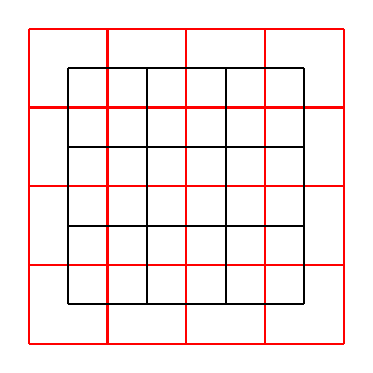
\begin{tikzpicture}
        \draw[step=1.0,thick,red] (0,0) grid (4,4);
        \draw[step=1.0,black,thick,shift={(0.5,0.5)}] (0,0) grid (3,3);
    \end{tikzpicture}
    \caption{The slots for generating a $3\times3$ tile world. Tiles are drawn in black, slots in red.}
    \label{fig:tiles-and-slots}
\end{center}

One example of such module is shown in figure~\ref{fig:wfc-module}.
Each module constrains the 8 adjacent slots.
An edge type is specified for each edge, and modules which share an edge must have the same edge type.
For each corner of the module, several tile constraints are specified.
The modules that share a tile must agree on the tile's properties: its height, slant direction (if any) and surface type.
Terrain types can have multiple surface types, each with a different set of modules and a few modules that allow to transition between them.
For example, a \emph{shore} module could have \emph{ground} tiles on one side and \emph{water} tiles on the other.
For each terrain type, it is also specified which surface types and which edge types block paths.

\begin{center}
    \captionsetup{type=figure}
    \begin{minipage}{.5\textwidth}
        \centering
        \includegraphics[width=0.95\textwidth]{img/Module model.png}
    \end{minipage}%
    \begin{minipage}{.5\textwidth}
        \centering
        \includegraphics[width=0.95\textwidth]{img/Module constraints.pdf}
    \end{minipage}
    \caption{An example module and its constraints.}
    \label{fig:wfc-module}
\end{center}

In figure~\ref{fig:wfc-modules}, we show 7 modules as an input.
However, when designing them, it would make more sense to think of them as 3 different modules that can each be rotated.
Thus, the modules we use will also have an option to select the allowed reflection and rotations.
Then, before generating the terrain, we will automatically generate all variants of each module.
Each module can also be placed at different height levels, which is handled similarly.
For example, the module shown in figure~\ref{fig:wfc-module} will effectively become 24 different modules in a terrain type with 4 height levels (0, 1, 2, 3), because it has 8 different reflections and rotations, and it can appear at 3 different height levels (0--1, 1--2, 2--3).

For each module, we also specify a weight.
This dictates how likely it is to be selected when collapsing a slot, compared to other modules.
For example, when we collapse a slot that only has two valid modules, with weights 1 and 4, then the first module will be selected with a 20\,\% probability.

We have decided to implement backtracking to solve contradictions.
If the algorithm only ever has to backtrack once before collapsing another slot, we say that it needs backtracking depth 1.
However, it is possible that the algorithm collapses a slot, finds a contradiction, and after backtracking, removes the only remaining module in the slot that was collapsed.
Thus, it creates another contradiction, which causes it to backtrack deeper.
We run some quick tests with the set of modules which is going to be used to generate terrain in the demo version.
During these tests, we were unable to generate a single world, without running into a contradiction.
However, most worlds only ever needed backtracking depth of 1 to successfully generate.
After that, we ran into diminishing returns.
Of the worlds that required backtracking depth 2, most required backtracking depth greater than 10.
So we decided to allow for backtracking depth 1 and otherwise just restart the generation, which makes it faster on average.

\xxx{I should probably provide the data I measured. Do I also need to explain the whole setup to make it reproducible?}

We also need to decide which slot to collapse at each step of the algorithm.
Merrell uses in their thesis a sort of scan line order, collapsing them in the lexicographic order of their coordinates.
This could theoretically introduce a directional bias in the results.
Gumin in their implementation always collapses a slot with the lowest \emph{Shannon entropy}.
However, from our testing, the results tend to look unnatural, often creating rectangular regions at the same height or repeating patterns.

To make the results more natural, we chose to select the slot at random.
This means that the generator first sets slots in various parts of the world to different heights.
Then it has to somehow connect these to make the world follow the rules we set.
This leads to more diverse results, however, the failure rate becomes very high, leading to slower generation.

As a compromise, we chose to weight the slots by the number of invalid slots $+\,1$.
This is an approximation of entropy that is trivial to compute, making it more likely to select more constrained slots, but still collapsing unconstrained slots once in a while.
The 1 is added just to make all weights nonzero.
This leads to results similar to the ones with uniform randomness, but decreases the failure rate substantially.

\xxx{Can I show screenshots of the generated worlds with different settings?}
\xxx{More testing data to compare the success rate of different approaches}

\subsection{Time Complexity of Na\"{i}ve WFC}\label{sec:wfc-time-complexity}

In this section, we will show that algorithm~\ref{alg:wfc} runs in amortized $O(k^3 \cdot n)$ time, where $k$ is the number of modules, and $n$ is the number of slots.
We will assume that the sets $uncollapsed$, $to\_update$ and the $modules$ of each slot have amortized $O(1)$ queries, additions and removals (including \textsc{Pop}).
Another assumption we will is that \textsc{IsValid} runs in $O(k)$ time, because each slot has $O(1)$ neighbors and each neighbor can only have $k$ different modules, so we have to check at most $O(k)$ constraints.

This means that checking the modules a slot can have takes $O(k^2)$ time.
Since each change removes at least one module, each slot can change up to $k$ times, and each change leads to $O(1)$ neighbors being checked.
There are only $n$ slots which means at most $kn$ changes, which means constraint propagation takes $O(k^3 \cdot n)$ time over the execution of the whole algorithm.

All other steps can are asymptotically faster:
Initialization is done in $O(kn)$ time.
Collapsing $n$ slots takes $O(kn)$ time, assuming picking the random module takes $O(k)$ time.

\section{Resources and Obstacles}

- after terrain generation, place blockers on tiles

- materials for the player to mine

- just rocks for variety - the player cant build on these

- set up as a few layers

- each stage has:

- one or more types of blocker (e.g. ore, small rocks, big rocks)

- *min* and *max* amounts

- *base chance* to place

- whether they can be placed on slanted tiles

- which surface Types they can be on (currently there is only one)

- *forces* - effect on chance based on already placed blockers

- for example: negative force with magnitude *m* from stage *s* means the chance to place a blocker on a given tile is decreased by *m/d*  for each blocker placed in stage *s*, where *d* is its distance from the considered tile

- for each stage:

- repeat until at least min blockers have been placed (in this stage)

- for each tile without a path or blocker (in random order):

- if random number between 0 and 1 < modified chance:

- place the blocker of the given type

- if there are max blockers (placed in this stage), end the stage

- scattering models

- unity physics engine X

- parallel

For the blockers, I didn't want repetitive obstacle models, so they are generated proceduraly by scattering many simpler models (decorations) on each tile

- first compute weights based on various factors (images!!!)

- distance to path

- height

- distance to other blockers

- customizable thanks to modular approach

- then scatter decorations in stages, each stage again having one type of decoration and many parameters

- for each tile in random order repeat x (specified for this stage) times:

- pick a random position within it

- calcualte the weight at this position (based on settings)

- check that it is greater than some threshold (based on settings)

- calculate the minimum distance to other decorations (from weight, based on settings)

- check that the position is far enough from other decorations

- calculate the decoration size (from weight, based on settings)

- place the decoration on this position, with the given size

\section{Terrain Types}

- what information is tied to the type

- why txt (inspector was not as legible)

\section{World Builder}

- builds the world from the generated data, it needs to be done in the main thread

- the rest will be in background threads

\section{Attacker Wave Generation}

- creates a randomized plan of waves

- two types of waves

- combine different attackers in sequence

- combine different attackers in parallel (only possible with multiple paths, rarer)

- each wave gets some throughput budget and buffer

- each attacker has a given cost

- when planning a wave, select attackers and spacing, such that the througput budget is exceeded

- for each attacker subtract the throughput overshoot from buffer

- fit such that as much of buffer gets used without going over

- branching

\section{Simulation}

- use fixed updates for game logic

- why?

- 20Hz = fixed time step 0.05s

- options to speed up or possibly pause - changing fixed update rate - not yet implemented

\section{Visuals and Interpolation}

- interpolate positions and visuals on Update

- many visuals are game-speed agnostic     - TODO: use unscaledDeltaTime

- I thought about some custom mini-framework for this, but many of the simulated variables the visuals are based on should be handled on case-by-case basis

\section{Attacker Targeting}

- Towers use it to acquire targets

- handles which Attackers are in range and which one is chosen as the current target

- can require line of sight to the enemy

- different targeting types

- rotation

- heights

- possibly ensure a trajectory

- preferred target (configurable)

- composite colliders

\section{Range Visualization}

- IMAGES!!

- Draw the range on the terrain mesh

- Draw on which parts of paths will Attackers be targeted

- green - all sizes

- yellow - only large

- Terrain shader uses compressed texture format instead of raw texture

- Options:

- quadrant compression format, 2bytes per node

- less CPU time, because the data is already in this format

- up to 48KiB per frame

- more GPU time

- 256x256 texture, 1byte per pixel

- more CPU time

- 64KiB per frame

- fast on GPU

- only 1 channel - cannot interpolate

- mipmaps -> one additional state

- less CPU time

- 33\% more data

- more pixels per byte

- possible future optimization

- less data

- more difficult indexing and stuff both on CPU and GPU

- interpolation could work with more than one channel and without mipmaps

\section{Game Commands}

- we want various components to modify how other components function

- examples

- also react to events as a bonus

\section{Blueprints}

- separation of stats from behavior

- why are they implemented this way

\subsection{Attacker Stats}

- blueprints for attackers

\subsection{Dynamic Descriptions}

- explain what things do and their stats

- attackers and blueprints

- dynamically reflect the changes made by other components
